\chapter{今後の展望}
\label{chapter5}
最後に、本論文の研究に関して今後期待される展望とGroundBIRDの今後のアップデートの方針について述べる。
\section{大気揺らぎに由来するノイズのモデリング}
\label{atmos_model}
\ref{chapter4}章でスキャン軸上の検出器がより高い相関を持つこと、すなわちより同じ大気を観測するように改善されたことを見た。また、図\ref{compare_9011_11139}や図\ref{compare_9011_11679}にあるように、検出器間の相関の違いが\SI{10}{Hz}前後で顕著に出る結果を得た。この結果から大気放射ノイズは\SI{10}{Hz}前後の周波数で観測されていると考えられる。大気の揺らぎは非常に複雑であり、大気を何かしらのモデルによって単純化することが必要になる。本研究で、異なる検出器配置とその配置での相関の差を得られたため、両者の結果を矛盾なく説明する大気のモデル(大気の揺らぐ時間的、角度的スケール)を構築することができれば、GroundBIRDで観測する大気ノイズに対する系統的な理解を深めることが期待できる。ノイズの性質をより理解できれば、観測データから適切にノイズを差し引くことができ、CMBの偏光をより高精度に観測することにつながる。

ここでは、\cite{nishinomiya}の大気モデルを参考に、大気の相関に関する簡易的な考察を行う。大気のモデルとして、図\ref{atmos_layer}のように平面的な大気の層が重なっているものを考える。

\begin{figure}[htbp]
  \centering
  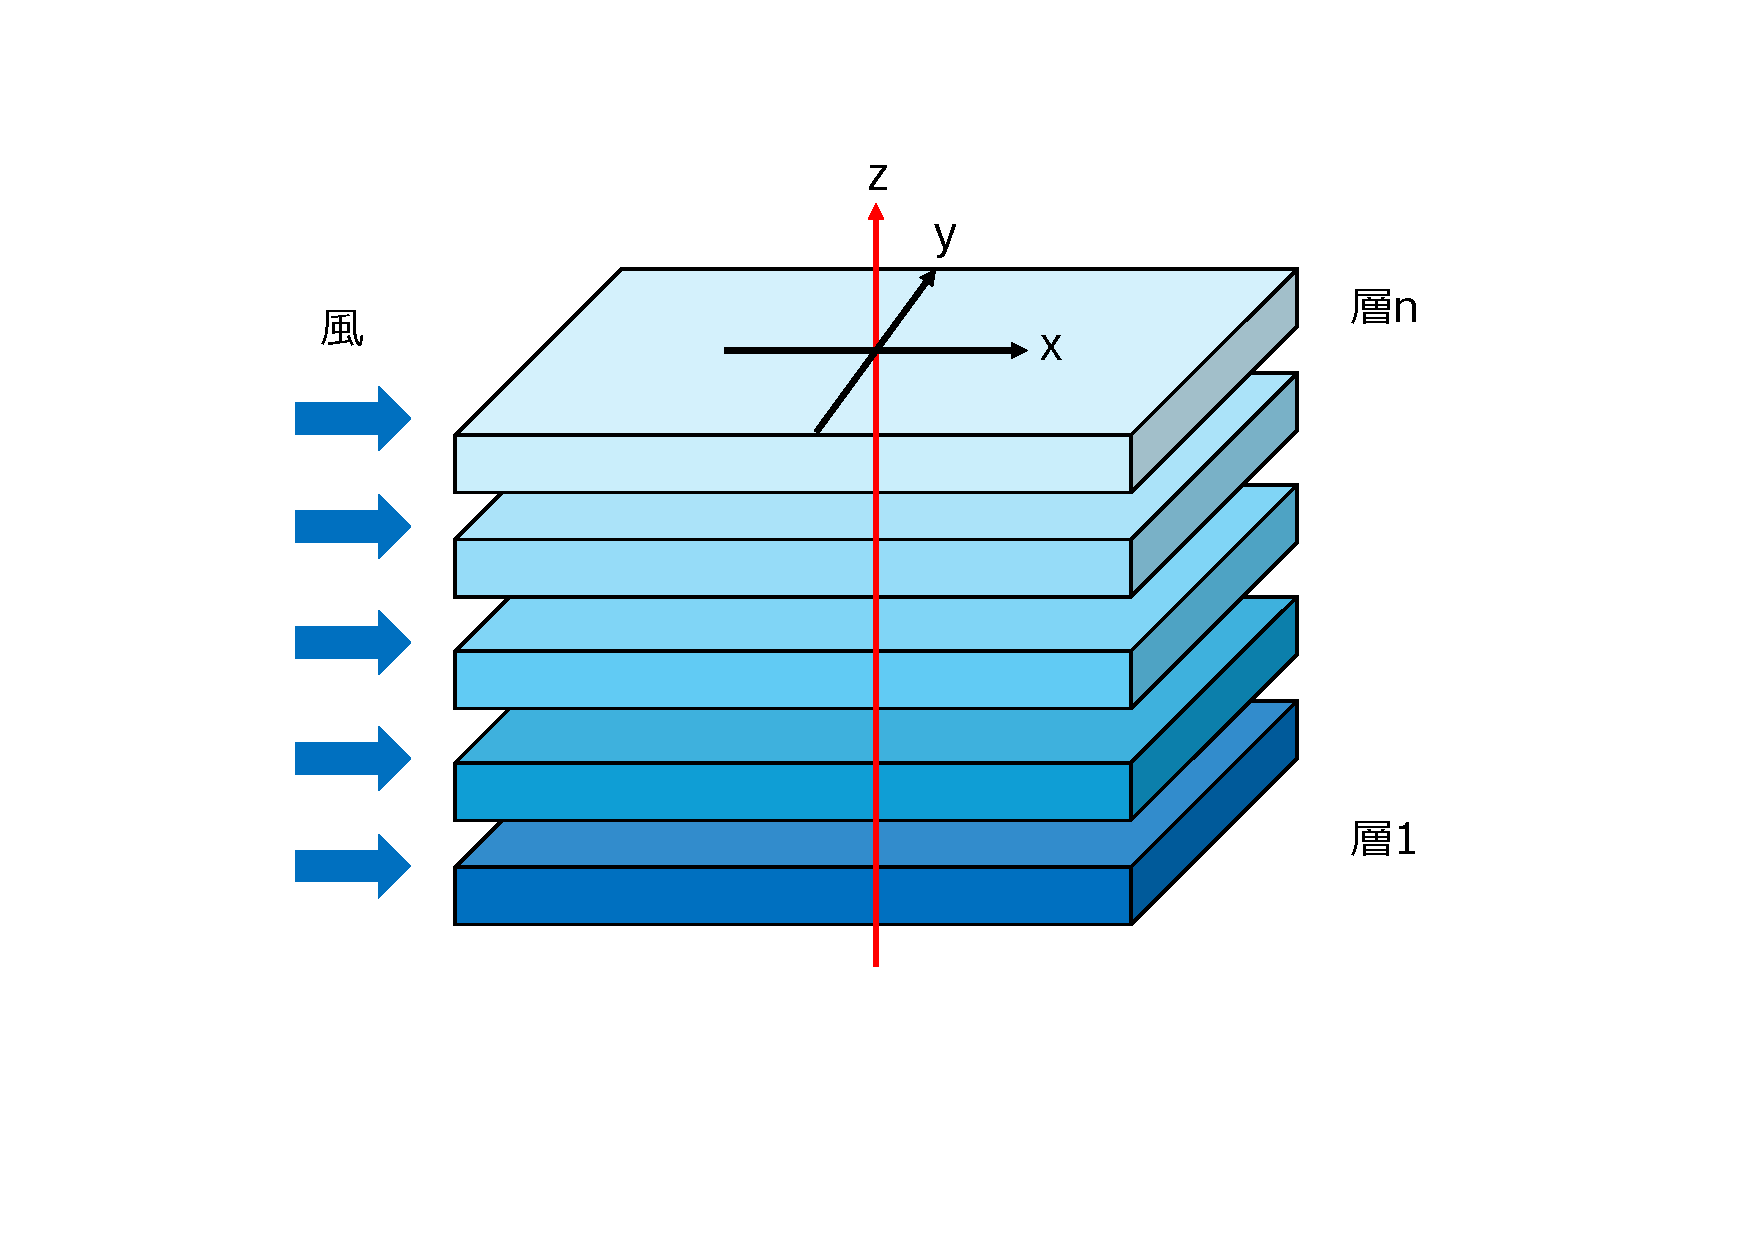
\includegraphics[width=0.7\columnwidth]{6_prospect/figs/atmos_layer.pdf}
  \caption{平面の層を用いた大気のモデル。全ての層は同じ風速の風を同じ方向に受けて動くと仮定している。}
  \label{atmos_layer}
\end{figure}
まず1層のみの場合で考える。層上の2つの検出器$i, j$があり、これらの座標の差を
\begin{equation}
  \Delta\bm{x} = (x_{i} -x_{j}, y_{i} - y_{j}) = (\Delta x, \Delta y)
\end{equation}
とする。この検出器間の相関を表す相関関数を
\begin{equation}
  R(\Delta\bm{x},\omega,z, v_{w}) = \frac{1}{2^{1/3}\Gamma(\frac{4}{3})}\mathrm{exp}\Bigl(i\frac{\omega}{v_{w}}\Delta x\Bigr)\Bigl(\frac{\omega}{v_{w}}|\Delta y|\Bigr)^{4/3}K_{4/3}\Bigl(\frac{\omega}{v_{w}}|\Delta y|\Bigr)
\end{equation}
と記述できる。ここで、$\omega$は周波数、$v_{w}$を風速、$K_{4/3}$は修正ベッセル関数を表す。
\section{両偏波アンテナを搭載した焦点面検出器のアップデート}
